\subsection{预测型/计数型模型}
按照训练的目标函数来分,词向量模型可分为两大类:
预测型模型(prediction-based)和计数型模型(count-based)。
预测型模型通常直接在原始文本上训练。
当一个上下文窗口(context window)扫描
文本时,模型通过上下文词预测中心词并最大化对数概率的似然度
(likehood of log probability)。
代表性的预测型有CBOW,Skip-gram及其扩展。
计数型模型则在文集的(正则化后的)词--词共现矩阵上训练,
直接从词共现数据中获取词向量。
代表性的计数型模型有Glo~Vec和LSA。

\subsubsection{预测型模型}

\paragraph{模型体系结构}
\begin{figure}
  \centering
  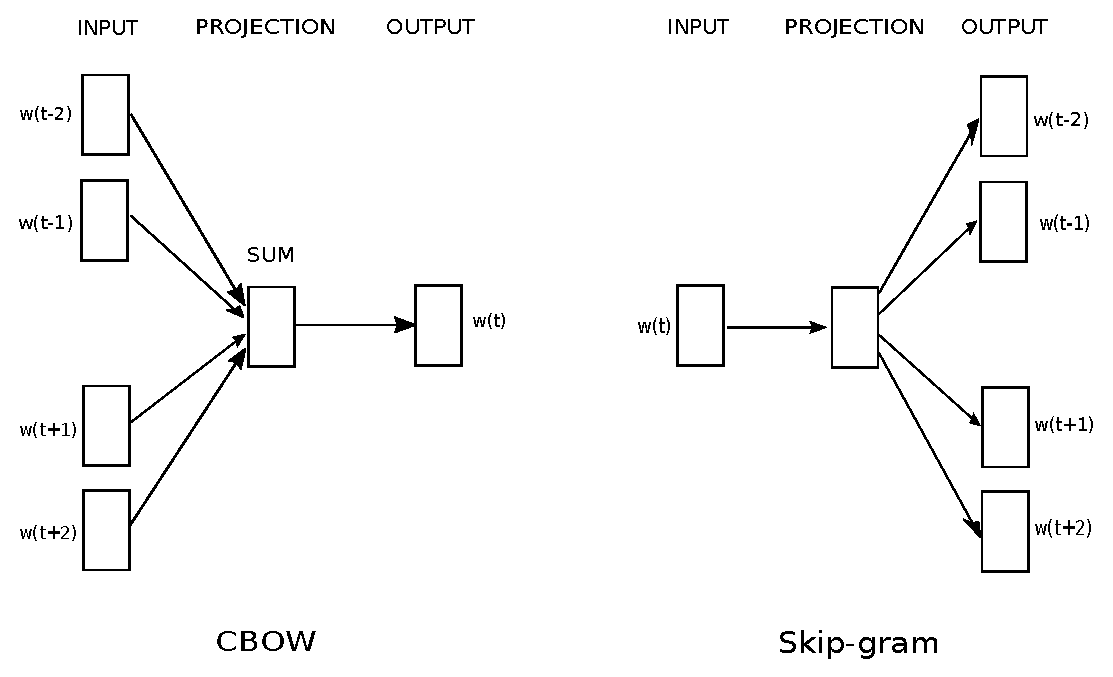
\includegraphics[width=\textwidth]{figures/word2vec-architecture.eps}
  \caption{CBOW和skip-gram的体系结构\cite{DBLP:journals/corr/abs-1301-3781}}
  \label{fig:word2vec-arch}
\end{figure}

预测型模型通常在一个上下文窗口内进行词预测,根据预测的结果调整模型的参数。
这类模型实际上在最大化如下对数概率的似然度:
\begin{align}
  J = - \sum_{\substack{i \in corpus \\ j \in context(i)}} \log Q_{ij}
\end{align}
其中,目标词为$w_i$,上下文词为$\tilde{w}_j$,$Q_{ij}$为
文集中任意一个窗口中的任意一个词出现的概率:
\begin{align}
  Q_{ij} &= \frac{\exp(w_i^T \tilde{w}_j)}
  {\sum_{k=1}^V \exp(w_i^T \tilde{w}_k)}
\end{align}

具体的,CBOW和Skip-gram的体系结如 \cref{fig:word2vec-arch} 所示。
以CBOW为例,设$b$是上下文窗口的大小,$w$表示单词,$\vec{w}$表示词向量。
CBOW在给定周围词向量$\vec{w}_{-b}, \cdots, \vec{w}_{-1}, \vec{w}_1, \vec{w}_b$的情况下预测中心词$w_0$。
首先计算上下文向量$\vec{c} = \frac{1}{2b} \sum_{i \in [-b,b]-\{0\}}\vec{w}_i$,
然后通过输出矩阵$\vec{O} \in \mathcal{R}^{|V|\times d_w}$
把上下文向量$\vec{c}$映射到待预测词的$|V|$维向量表示。
通过反向传播,最大化如下概率:
\begin{align}
  p(\vec{v}_0|\vec{w}_{[-b,b]-\{0\}}) = \frac{\exp \vec{v}_0^T \vec{Oc}}{\sum_{\vec{v} \in V} \exp \vec{v}^T \vec{Oc}}
\end{align}

\paragraph{计算复杂度}
预测型模型以在线的形式扫描整个文集,因此复杂度和文集的大小成正比:
\begin{align}
  \mathcal{O} = E \times T \times Q
  \label{eqn:predict-based-complexity}
\end{align}
其中,$E$为训练的迭代次数,$T$为文集的大小,$Q$是一个与模型相关的复杂度。

对于CBOW,$Q$为:
\begin{align}
  Q = N \times D + D \times \log_2(V)
  \label{eqn:cbow-complexity}
\end{align}
其中$N$为窗口大小,$D$为词向量的维度,$V$为词汇表的大小。

对于Skip-gram,$Q$为:
\begin{align}
  Q = C \times (D + D \times \log_2(V))
  \label{eqn:skip-gram-complexity}
\end{align}
其中$C$是词的最大距离。

\paragraph{讨论}
优点:模型简单高效,可以在大文集上训练维度较高的词向量;
习得的词向量具有良好的语法和语义性质;
缺点:CBOW忽视了上下文词的顺序,导致词向量的语法性质较差。
Skip-gram对窗口大小的扩展性较差,窗口增大一个词导致模型多做两次
预测,每次的操作数是$D \times V$\cite{DBLP:conf/emnlp/LingTAFDBTL15}。

\subsubsection{计数型模型}
计数型模型先把文集中的共现信息收集到一个词--词共现矩阵中,然后从该矩阵学习词向量。
计数型模型的例子有\cite{DBLP:journals/jasis/DeerwesterDLFH90}和\cite{pennington2014glove}。
下面以Glo~Vec模型为例介绍计数型模型。

\paragraph{模型的出发点(Intuition)}
Pennington等人观察到,在大文集中,共现概率的比例(ratio of co-occurrent probability)可以反映词和词的相似关系。
设词--词共现计数矩阵为$X$,元素$X_{ij}$表示词$j$在词$i$的上下文出现的次数。
令$X_i = \sum_k X_{ik}$为任何词在词$i$的上下文出现的次数。
令$P_{ij} = P(j|i) = X_{ij}/X_i$为词$j$在词$i$的上下文出现的概率。
则对于一个上下文词$k$,根据$k$与$i,j$的相关性,
理论上可能出现的情况如 \cref{tab:glove-similarity-ratio} 所示。

\begin{table}
  \setlength{\columnsep}{8pt}
  \renewcommand{\arraystretch}{1.5}
  \centering
  \caption{词相关性与共现概率比例的关系}
  \label{tab:glove-similarity-ratio}
  \begin{tabular}{@{\quad}l@{\quad}l@{\quad}}
    \toprule
    $k$与$i,j$的相关性 & $P_{ik}/P_{jk}$ \\
    \midrule
    只与$i$相关 & 远大于1  \\
    只与$j$相关 & 远小于1  \\
    与$i,j$都不相关 & 接近1  \\
    与$i,j$都相关 & 接近1  \\
    \bottomrule
  \end{tabular}
\end{table}

Pennington等人以热力学词汇ice和steam为例,在大文本上测定了上述比例
(如 \cref{tab:glove-corpus-ratio} 所示),得出的数据和理论分析吻合。
这表明共现概率的比例包含着词的分布式含义,可以作为训练词向量的数据来源。

\begin{table}
  \setlength{\tabcolsep}{8pt}
  \renewcommand{\arraystretch}{1.5}
  \centering
  \caption{词ice和steam的共现概率,
    上下文选自一个60亿的文集。
    比1大得多的值表示和ice的相关性较强,
    比1小得多的值表示和steam的相关性较强。
  \cite{pennington2014glove}}
  \label{tab:glove-corpus-ratio}
  \begin{tabular}{l|cccc}
    Probability and Ratio & $ k = solid $ & $ k = gas $ & $ k = water $ & $ k = fashion$ \\ \hline
    $ P(k |ice)$ &$ 1.9 \times 10^{-4} $&$ 6.6 \times 10^{-5} $&$ 3.0 \times 10^{-3} $&$ 1.7 \times 10^{-5}$\\
    $ P(k |steam)$ &$ 2.2 \times 10^{-5} $&$ 7.8 \times 10^{-4} $&$ 2.2 \times 10^{-3} $&$ 1.8 \times 10^{-5}$\\
    $ P(k |ice)/P(k |steam)$ &$ 8.9 $&$ 8.5 \times 10^{-2} $&$ 1.36 $&$ 0.96$\\
  \end{tabular}
\end{table}

\paragraph{模型体系结构}
基于上述观察,Pennington等人提出了一个一般的模型:
\begin{align}
  F(w_i,w_j,\tilde{w}_k) = \frac{P_{ik}}{P_{jk}}
  \label{eqn:glove-general}
\end{align}
其中等式的右边从训练数据中获取;$F$是一个任意函数。
为了得出具体的目标函数,
Pennington等人对 \cref{eqn:glove-general} 加入了限制条件并进行变形,
过程如 \cref{tab:glove-constrains} 所示。最后得出的目标函数为:
\begin{align}
  J = \sum_{i,j=1}^V f\left(X_{ij}\right) \left(w_i^T\tilde{w}_j+b_i+\tilde{b}_j-\log(X_{ij})\right)^2
  \label{eqn:glove-objective}
\end{align}

\begin{table}
  \setlength{\tabcolsep}{6pt}
  \renewcommand{\arraystretch}{1.5}
  \centering
  \caption{对 \cref{eqn:glove-general} 施加的限制条件及其理由}
  \label{tab:glove-constrains}
  \begin{tabular}{p{0.25\textwidth}p{0.25\textwidth}p{0.45\textwidth}}
    \toprule
    限制条件 & 理由 & 公式变形 \\
    \midrule
    $F$应作用于$w_i, w_j$的向量差 & 词的含义由向量差编码 &
    $\begin{aligned}
      F(w_i - w_j, \tilde{w}_k) = \frac{P_{ik}}{P_{jk}}
    \end{aligned}$ \\
    $F$应对两个参数取内积 & 内积是线性函数,保留了参数的线性性 &
    $\begin{aligned}
      F\left(( w_i - w_j )^T \tilde{w}_k\right) = \frac{P_{ik}}{P_{jk}}
    \end{aligned}$ \\
    等式应在交换$w \leftrightarrow \tilde{w}, X \leftrightarrow X^T$下
    保持成立 & 在$X$中目标词和上下文词是对称的 &
    $\begin{aligned}
      F(w_i^T\tilde{w}_k) = P_{ik} &= \frac{X_{ik}}{X_i}, F=\exp \\
      w_i^T\tilde{w}_k = \log(P_{ik}) &= \log(X_{ik}) - \log(X_i) \\
    \end{aligned} $ \\
    把$\log(X_i)$作为偏置$b_i$并增加$\tilde{b}_k$ & 恢复偏置的对称性 &
    $\begin{aligned}
      w_i^T\tilde{w}_k + b_i + \tilde{b}_k = \log(X_{ik})
    \end{aligned}$ \\
    \bottomrule
  \end{tabular}
\end{table}

其中,$f(X_{ij})$是一个加权函数,它的作用与性质如 \cref{tab:glove-weight-reasons} 所示。
Glo~Vec模型采用的加权函数为:
\begin{align}
  f(x) = \begin{cases}
    (x/x_{max})^\alpha \quad &\text{if } x < x_{max} \\
    \quad\quad 1 \quad &\text{otherwise} \\
  \end{cases}
  \label{eqn:glove-weight}
\end{align}
从 \cref{fig:glove-weight-fn} 上看,该函数满足 \cref{tab:glove-weight-reasons} 的要求。
Pennington等人进一步指出,当$x_{max} = 100$,$\alpha = 3/4$时,模型的性能最好
\cite{pennington2014glove}。

\begin{table}
  \centering
  \caption{加权函数$f(X_{ij})$的作用和性质}
  \label{tab:glove-weight-reasons}
  \begin{tabular}{m{0.5\textwidth}m{0.5\textwidth}}
    \toprule
    作用 & 性质 \\
    \midrule
    消除对数函数当$x \rightarrow 0$时的发散性 &
    $\lim_{x\rightarrow 0} f(x) = 0$且趋于0的速度应该足够让$lim_{x \rightarrow 0} f(x)\log^2x$是有限的 \\
    少见词的共现不会被赋以过大的权重 & 非减函数 \\
    频繁词的共现不会被赋以过大的权重 & 当自变量较大时,$f(x)$的值应该较小 \\
    \bottomrule
  \end{tabular}
\end{table}

\begin{figure}
  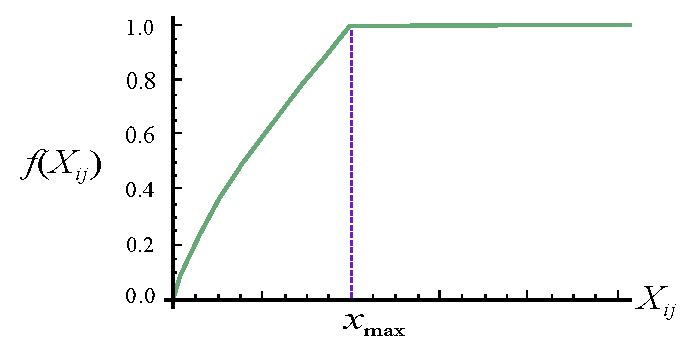
\includegraphics[width=0.8\textwidth]{figures/glove-weight.eps}
  \centering
  \caption{$\alpha=3/4$时的权重函数$f$}
  \label{fig:glove-weight-fn}
\end{figure}

\paragraph{计算复杂度}
计数型模型的计算复杂度包括建立词--词共现矩阵和训练模型两部分。
通过并行计算,建立$X$并不是一个计算瓶颈(参考\cite{DBLP:conf/eacl/LebretC14}的benchmark得知)。

训练模型的复杂度和$X$的非零元素数,词向量维度$D$和迭代次数$E$的乘积成正比:
\begin{align}
  O = |X_{non-zeros}| \times D \times E
  \label{eqn:glove-loose-bound}
\end{align}

其中,$|X_{non-zeros}|$是$X$的非零元素数,以矩阵的全部元素$|X|$(也就是$O(V^2)$)
为上界。粗略一看计数型模型似乎有着比预测型更大的复杂度,因为$|V|^2$
通常大于大部分的文集的大小$|C|$。
然而,假设$X$的元素$X_{ij}$的分布服从以词频等级(frequency rank)$r_{ij}$为底数的指数定律(power law):
\begin{align}
  X_{ij} = \frac{k}{(r_{ij})^\alpha}
\end{align}
我们获得了更紧的上界\footnote{推导从略}:
\begin{align}
  |X_{non-zeros}| = \begin{cases}
    \mathcal{O}(|C|) \ \quad\quad\text{if $\alpha < 1$,} \\
    \mathcal{O}(|C|^{1/\alpha}) \quad\text{if $\alpha > 1$.} \\
  \end{cases}
  \label{eqn:glove-tight-bound}
\end{align}
可见,当文集的分布规律满足$\alpha > 1$时,计数型模型的时间复杂度优于预测型模型。

\paragraph{讨论}
优点:模型清晰明了,目标函数中直接体现了向量偏移方法所衡量的性质。
模型训练高效,时间复杂度在一定程度上优于预测型方法。
在词类比任务上,模型的性能是训练时间的非减函数\cite{pennington2014glove}。
缺点:模型的最坏时间复杂度为$\mathcal{O}{|V|^2}$。
